\documentclass[a4paper,11pt]{ctexart}

\usepackage[margin=1in]{geometry}
% 调整页面大小,默认页面与常用规格不符

% 用来输入摘要
\usepackage{abstract}

% 用来插入图片
\usepackage{graphicx}

% 插入数学符号
\usepackage{amsmath}
\usepackage{amsfonts}
\usepackage{amssymb}
\usepackage{amsthm}

% 引用链接可点击
\usepackage{cite}
\usepackage[colorlinks,linkcolor=black,anchorcolor=blue,citecolor=green]{hyperref}

% 用于插入伪代码
\usepackage{clrscode3e}

% 用于插入C代码
\usepackage{listings}

% 调整代码的背景和风格
\usepackage{xcolor}
\lstset{
    %行号
    numbers=left,
    %背景框
    framexleftmargin=10mm,
    frame=none,
    %背景色
    %backgroundcolor=\color[rgb]{1,1,0.76},
    backgroundcolor=\color[RGB]{245,245,244},
    %样式
    keywordstyle=\bf\color{blue},
    identifierstyle=\bf,
    numberstyle=\color[RGB]{0,192,192},
    commentstyle=\it\color[RGB]{0,96,96},
    stringstyle=\rmfamily\slshape\color[RGB]{128,0,0},
    %显示空格
    showstringspaces=false
}

% 设置Section标题风格
\ctexset{
section={
    name={,、},
    number= \chinese{section},
    format = \raggedright,
}
}


% 部分使用说明
% \begin{lstlisting}[language={C}]
% 正式代码在此输入
% \end{lstlisting}

% \begin{codebox}
% 伪代码在此输入
% \end{codebox}

\begin{document}

\begin{titlepage}
\begin{center}

% 页面正中央插入的图片及哈尔滨工业大学英文全称

\includegraphics[width=0.8\textwidth]{./images/HIT.eps}\\[1cm]
\textsc{\LARGE Harbin Institute of Technology}\\[1.5cm]

% 标题
\hrulefill \\[0.4cm]
{ \huge \bfseries 数字逻辑大作业}\\[0.4cm]
\hrulefill \\[1.5cm]

% 作者和其他信息
\begin{minipage}{0.4\textwidth}
\begin{flushleft} \large

\end{flushleft}
\end{minipage}

% 右侧
\begin{minipage}{\textwidth}
\begin{flushright} \large
\emph{成员A:}冯云龙\\
\emph{学号:}1160300202\\
\emph{成员B:}赖\ \ \ 昕\\
\emph{学号:}1160300203\\
\end{flushright}
\end{minipage}

\vfill
{\large \today}% 底部插入当日日期
\end{center}
\end{titlepage}

\part*{摘要}大作业是在学完本门课程后,对所学知识的综合性考察. 知识覆盖面宽,实验所需时间长。要求学生灵活运用学过的计数器、触发器、译码电路等方面的知识,独立完成从设计、选片、连线、调试、排除故障到实现一个数字系统的全过程,详细书写项目报告。通过综合设计性实验,培养学生灵活运用所学知识解决比较复杂的实际问题的能力。
\paragraph{关键词:电子密码锁}

\tableofcontents            % 生成目录并隔开正文
\newpage

\part{正文}
\section{设计目的及要求}
\begin{enumerate}
\item 设计一个开锁密码至少为4位数字(或更多)的密码锁。
\item 当开锁按扭开关(可设置8位或更多,其中只有4位有效,其余位为虚设)的输入代码等于所设密码时启动开锁控制电路,并且用绿灯亮、红灯灭表示开锁状态。
\item 从第一个按扭触动后的5秒内若未能将锁打开,则电路自动复位并发出报警信号,同时用绿灯灭、红灯亮表示关锁状态。
\item 密码锁中的4位密码可以修改。
\item 记录按键次数并显示。
\item 倒计时。
\end{enumerate}

\section{工作原理、系统方框图}
\begin{center}
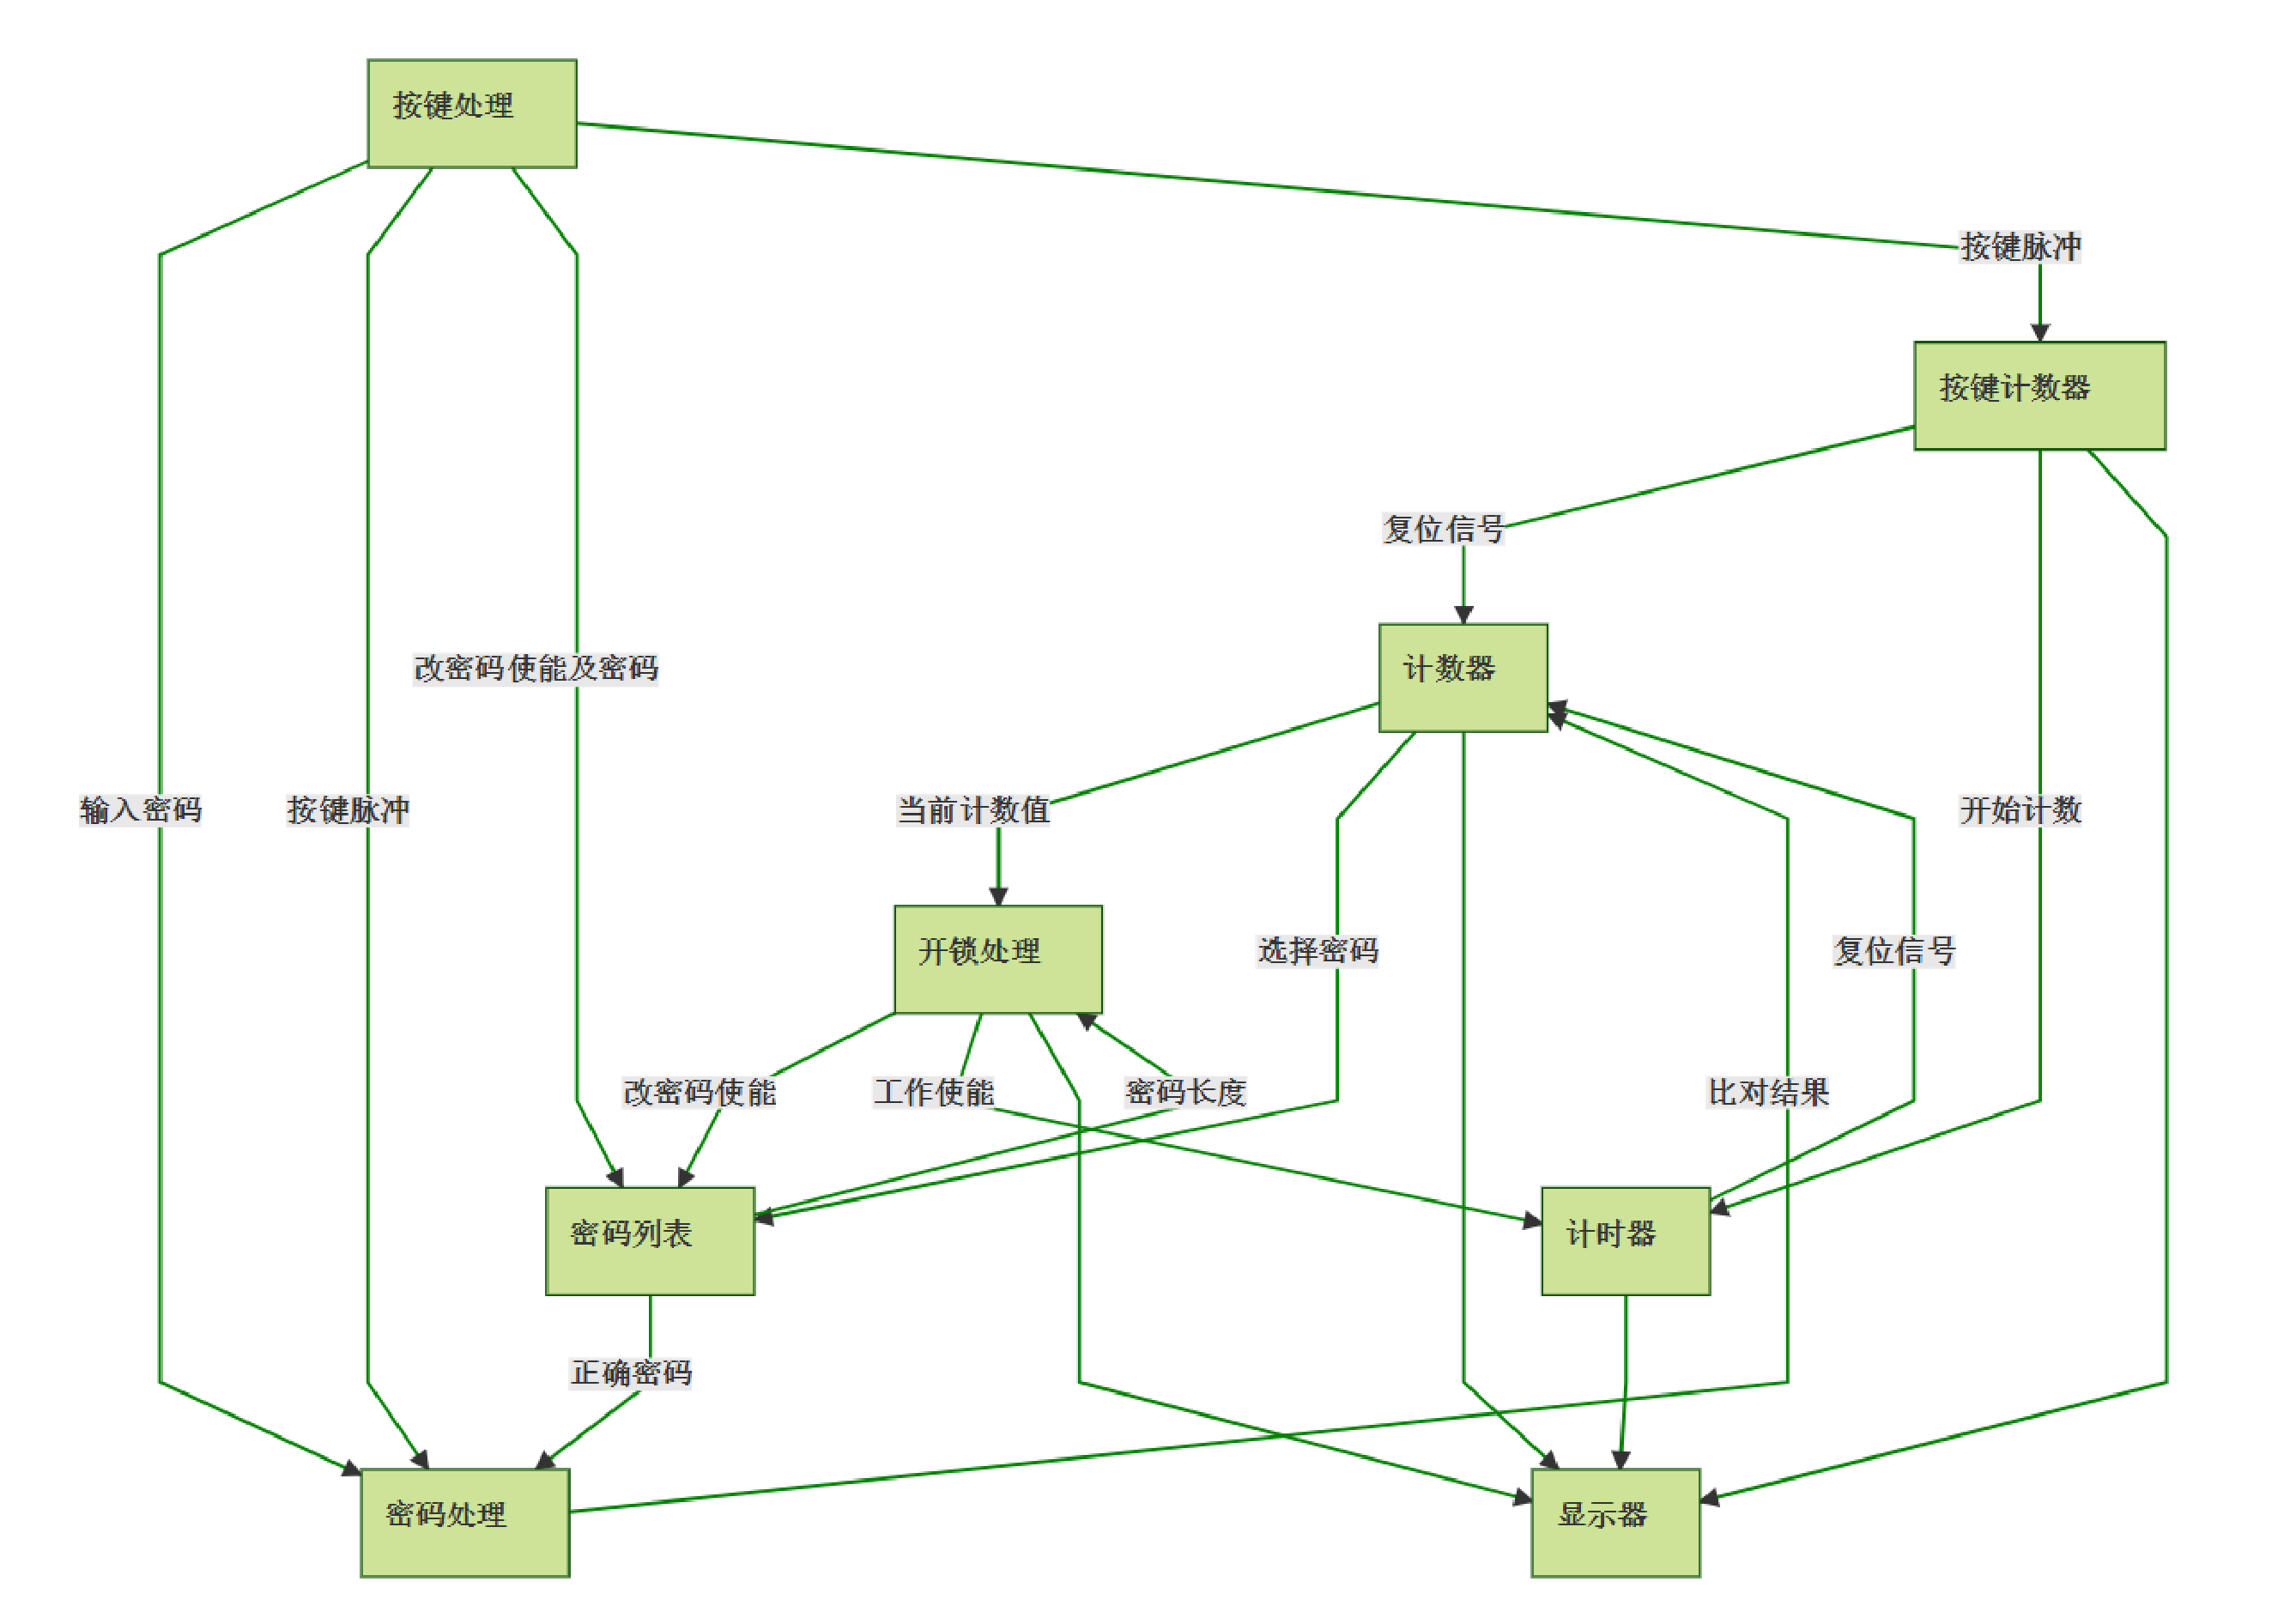
\includegraphics[width=0.9\textwidth]{./images/struct.eps}
\end{center}
\section{各部分选定方案及电路组成、相关器件}
\paragraph{密码处理}这部分我们使用的是一个等值比较器,对密码进行比对,当输入的密码与存储列表中的密码相等时,输出给计数器,使计数器计数。
\paragraph{密码表}首先我们使用了16位寄存器以储存密码和密码长度,使用数据选择器对数据进行选择,在开锁情况下,给予修改信号可以对密码进行修改,当使用计数器对每一位进行修改,可以通过关闭修改信号以停止修改,当不再修改密码时,自动复位。
\paragraph{密码计数器}串行输入密码,每输对一位密码,计一次数,可以通过按键计数器与计时器所给的复位信号进行复位(同步清零)。
\paragraph{开锁控制器}实际上是一个等值比较器,将密码计数器的值与设置的密码长度进行比较,若相等,则输出为1。
\section{调试过程}
\subsection{密码表中出现的问题}
\begin{enumerate}
  \item 变量未声明,经检查是变量名写错了,经过简单的修改就又可以正常工作了。

        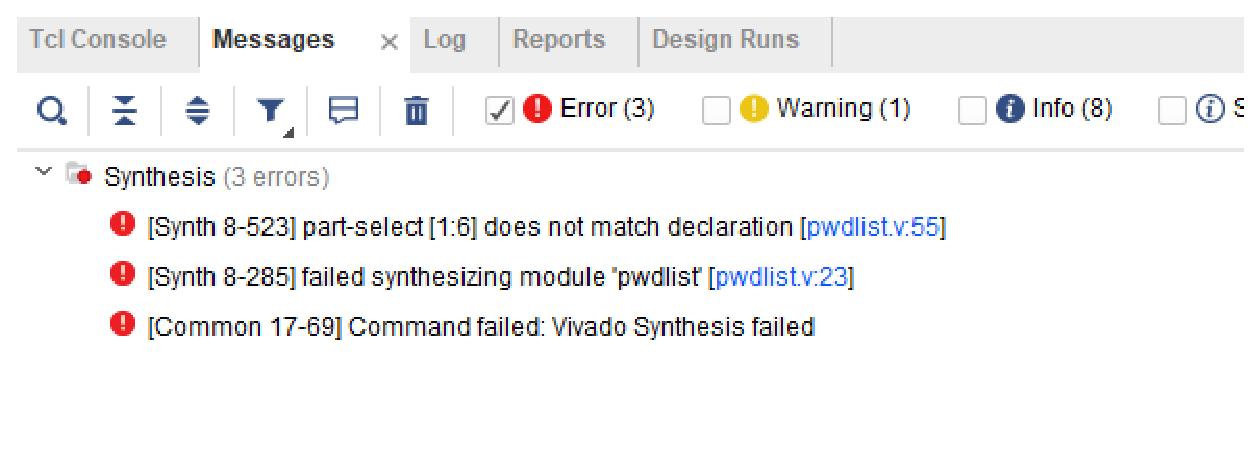
\includegraphics[width=0.9\textwidth]{./images/error0.eps}
  \item 这个错误很棘手,在百度时发现是由于在两个$always$块里修改了同一个$reg$变量,我对修改变量的部分做了综合,使用按键的上升沿进行触发,结果又出现了下面的错误。这也导致其无法自动复位。
        后来经过代码修改,使得在不修改密码时,密码长度计数值自动复位,又成功实现了自动复位。

        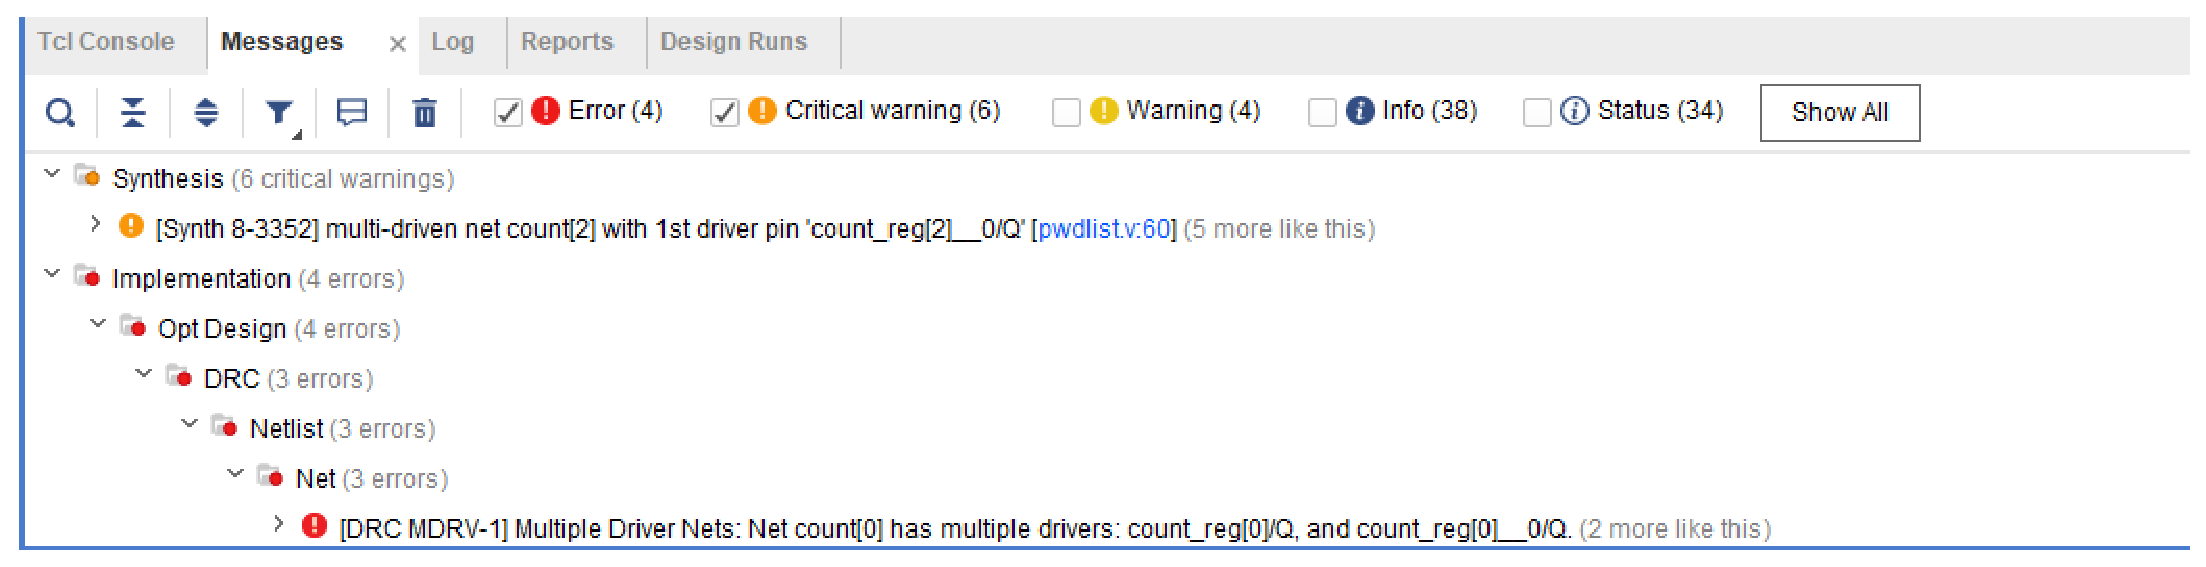
\includegraphics[width=0.9\textwidth]{./images/error4.eps}
  \item 这个错误中提到Pin$R15$不能当作CLK使用,多次研究后,将上升沿触发取消掉,成功。

        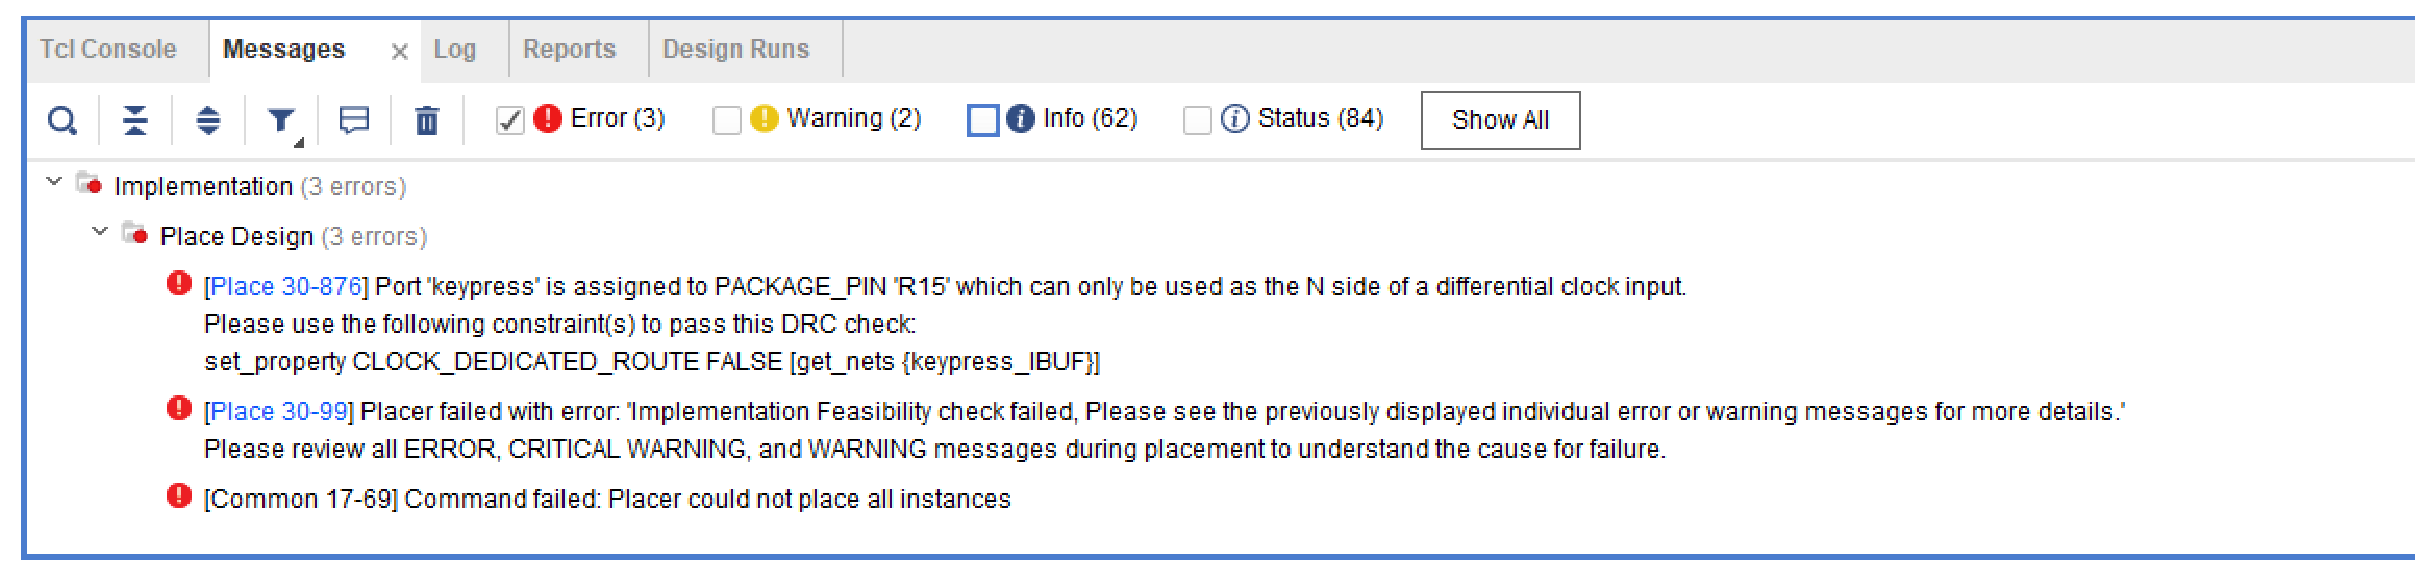
\includegraphics[width=0.9\textwidth]{./images/error5.eps}

  \item 中间调试过程中发现改了一位密码就会改变开锁状态,导致密码修改失败,经过修改,使得密码长度变更发生在密码更改完毕后,解决问题。
\end{enumerate}

\subsection{按键处理模块问题}
在按键处理模块中,需要编写延迟器使得按键脉冲能够为密码处理模块提供上升沿时钟信号。写完代码后进行仿真,发现其仿真波形图如下:

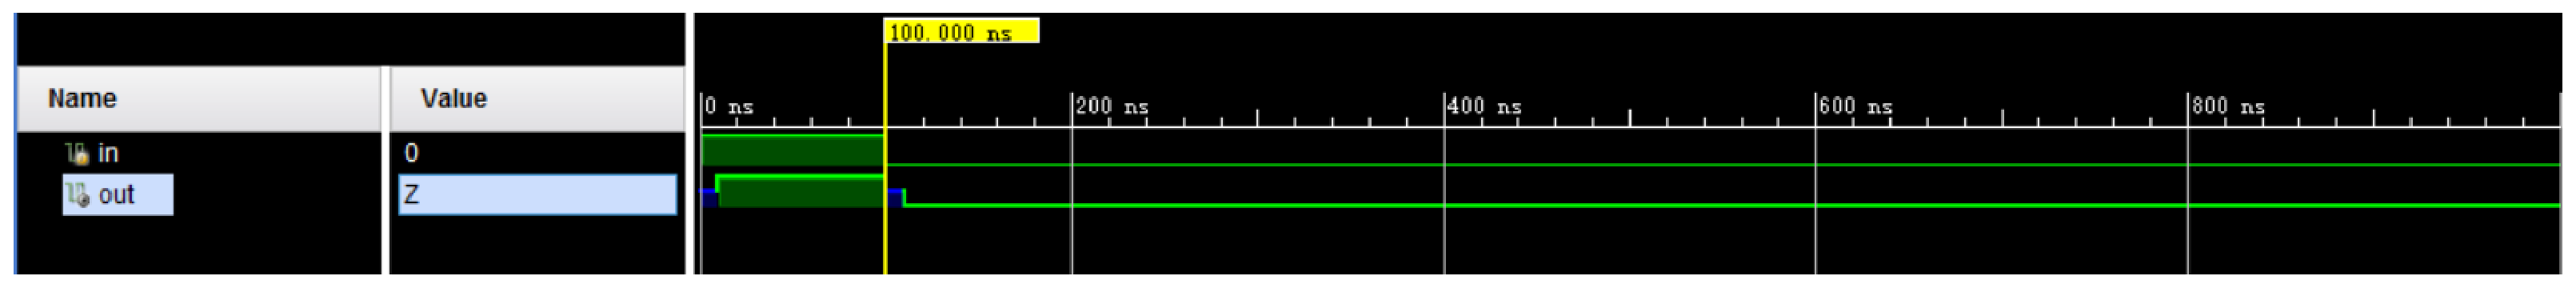
\includegraphics[width=0.9\textwidth]{./images/Lsim1.eps}

在in从高电平转为低电平之后的10ns内,out并没有延续in之前高电平信号,而是变成高阻态,过了10ns才成为低电平状态,延迟器代码出现问题,发现其实只需要在最初始的10ns内为高阻态即可,需要初始化。按照下图
修改之后,波形图为想要的图:

\includegraphics[width=0.4\textwidth]{./images/Lchange1.eps}
\includegraphics[width=0.4\textwidth]{./images/Lchange2.eps}

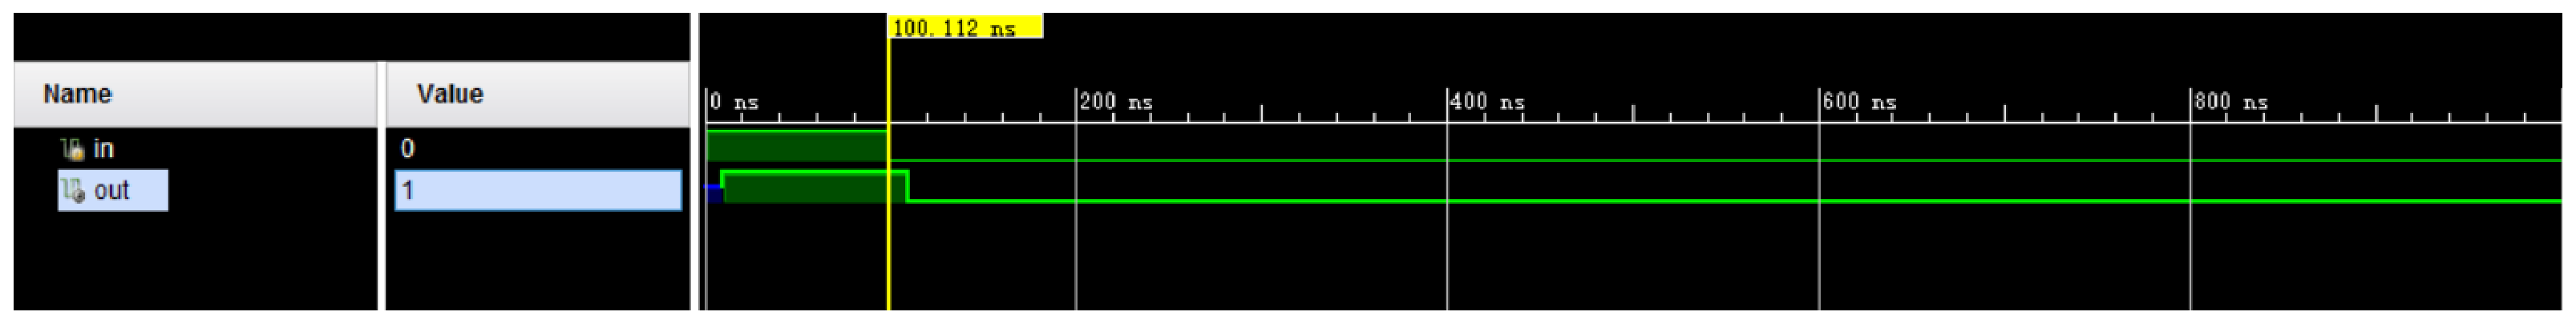
\includegraphics[width=0.9\textwidth]{./images/Lsim2.eps}

在按键计数器模块中,欲用D触发器拼装成一个模8计数器。在编写D触发器时需要异步低效清零端clr,写完代码后进行仿真,却发现自己写的竟然是同步高有效清零了。

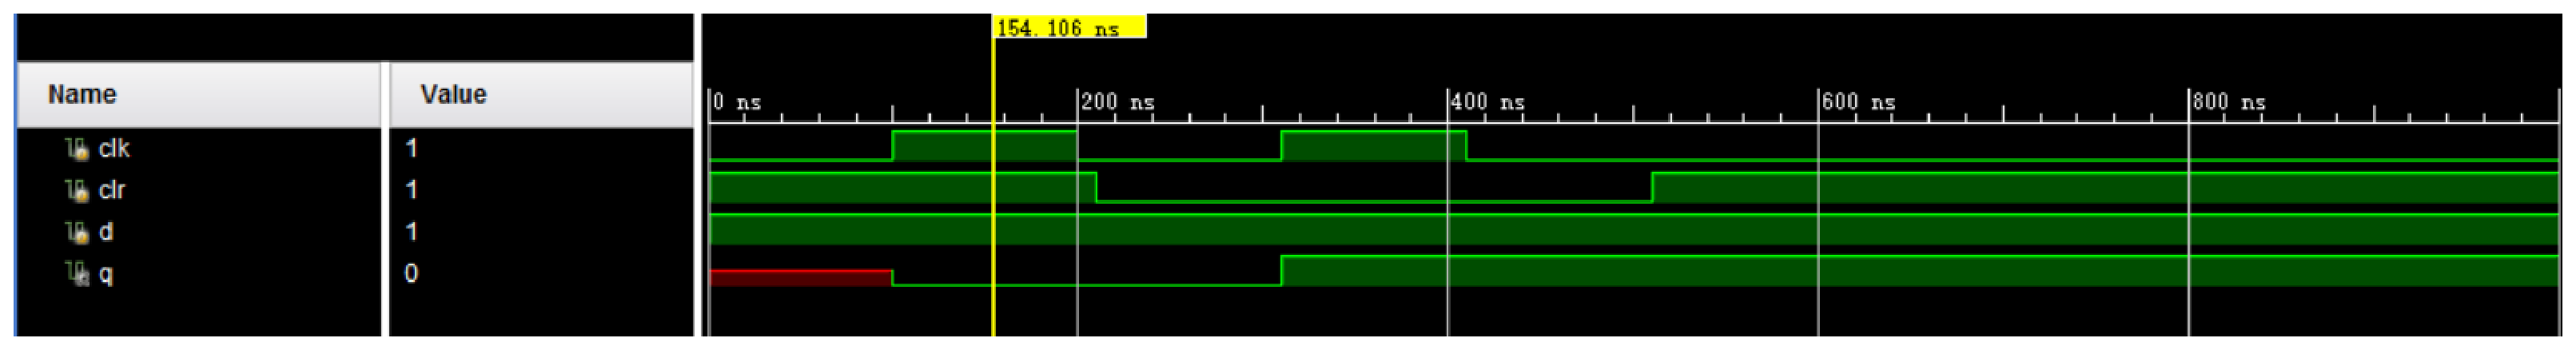
\includegraphics[width=0.9\textwidth]{./images/Lsim3.eps}

经过检查代码,发现在always块的敏感列表除posedge clk外未加clr,导致清零端同步时序。另外再将clr的有效值更改为0即可。
\section{设计结论}
\subsection{项目成果}
通过团队的分工与合作,我们完成了带有三个附加功能的密码锁。可以修改密码,通过按键计数和时间限制进行报警。
\subsection{项目团队}
我们的团队一共有两名成员,地位是等同的,分工协作完成了我们的项目。期间我们进行了各种讨论以敲定最终的接口。

\section{设计心得与总结}
\subsection{冯云龙}大作业的设计是曲折的,这次设计让我体会到设计接口的必要性,在设计整个项目的时候,我仿照着计算机界协同工作的一般形式,即先设计接口,再实现功能。
很多时候一个大的工程都不是一个人完成的,而是许许多多的人分工合作完成的,如何协调任务,分配任务是一个很重要的问题。计算机领域的解决方案就是设计接口,这样就隐藏了具体实现,只关注功能的可用性。
每一个模块在设计之初如果就完成了整合,那么每个模块只要按照文档实现,那么实现后一定也能很好的整合。这次的大作业,我们只有两个人,设计的重要性就已经体现出来,更大的工程项目肯定对于设计的要求会更高。
团队的合作,设计是极为重要的。
\subsection{赖昕}


\section{参考文献}

\begin{enumerate}
  \item verilog语言实现任意分频http://blog.csdn.net/ywhfdl/article/details/7641288
  \item verilog入门教程
  \item Tobias Oetiker,Hubert Partl, Irene Hyna and Elisabeth Schlegl,lshort-zh-cn
\end{enumerate}

\newpage
\appendix
\part{附录}
\section{总体器件表及相关器件的功能表、管脚分布}
\subsection{密码长度计数器}
\begin{figure}[htb]
  \begin{minipage}[b]{0.5\textwidth}
    \centering
    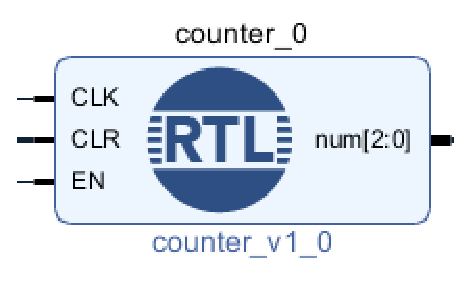
\includegraphics{./images/counter.eps}
    \caption{密码长度计数器}
    \label{fig:by:table}
  \end{minipage}%
  \begin{minipage}[b]{0.5\textwidth}
    \centering
    \begin{tabular}{|c|c|} \hline
      管脚名 & 功能                                            \\ \hline\hline
      CLK       &   上升沿触发计数      \\
      CLR       & 异步清零端                     \\
      EN        & 使能端                             \\
      num       & 当前密码输对的个数    \\ \hline
    \end{tabular}
    \caption{功能表}
    \label{table:by:fig}
  \end{minipage}
\end{figure}

\subsection{密码处理}
\begin{figure}[htb]
  \begin{minipage}[b]{0.5\textwidth}
    \centering
    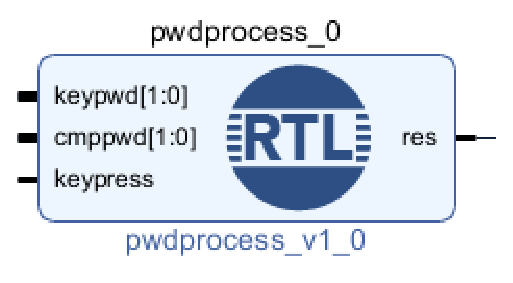
\includegraphics{./images/pwdprocess.eps}
    \caption{密码处理}
    \label{fig:by:table}
  \end{minipage}%
  \begin{minipage}[b]{0.5\textwidth}
    \centering
    \begin{tabular}{|c|c|} \hline
      管脚名 & 功能 \\ \hline\hline
      keypwd    &   按键输入密码 \\
      cmppwd    & 正确密码输入端 \\
      keypress  & 按键脉冲,有按键 \\
      res       &  比对结果 \\ \hline
    \end{tabular}
    \caption{功能表}
    \label{table:by:fig}
  \end{minipage}
\end{figure}

\subsection{开锁控制器}
\begin{figure}[htb]
  \begin{minipage}[b]{0.5\textwidth}
    \centering
    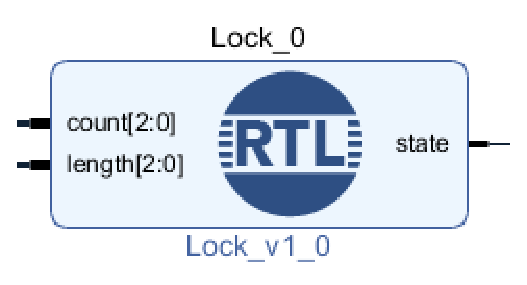
\includegraphics{./images/Lock.eps}
    \caption{开锁控制器}
    \label{fig:by:table}
  \end{minipage}%
  \begin{minipage}[b]{0.5\textwidth}
    \centering
    \begin{tabular}{|c|c|} \hline
      管脚名 & 功能 \\ \hline\hline
      count     &   当前输入正确密码的位数 \\
      length    &   正确密码总长度 \\
      state     & 当前开锁状态 \\ \hline
    \end{tabular}
    \caption{功能表}
    \label{table:by:fig}
  \end{minipage}
\end{figure}

\subsection{密码表}
\begin{figure}[htb]
  \begin{minipage}[b]{0.5\textwidth}
    \centering
    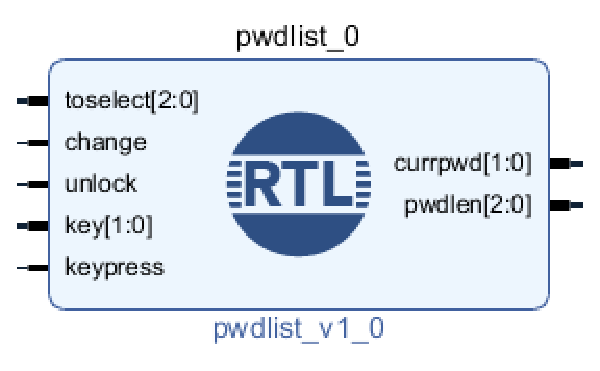
\includegraphics{./images/pwdlist.eps}
    \caption{密码表}
    \label{fig:by:table}
  \end{minipage}%
  \begin{minipage}[b]{0.5\textwidth}
    \centering
    \begin{tabular}{|c|c|} \hline
      管脚名 & 功能 \\ \hline\hline
      toseclect     &   选择的密码 \\
      change        & 是否修改密码 \\
      unlock        & 是否已开锁 \\
      key           & 按键值 \\
      keypress      & 按键脉冲 \\
      currpwd       & 当前正确密码\\
      pwdlen        & 密码长度 \\ \hline
    \end{tabular}
    \caption{功能表}
    \label{table:by:fig}
  \end{minipage}
\end{figure}

\subsection{按键部分}
\begin{figure}[htb]
  \begin{minipage}[b]{0.5\textwidth}
    \centering
%    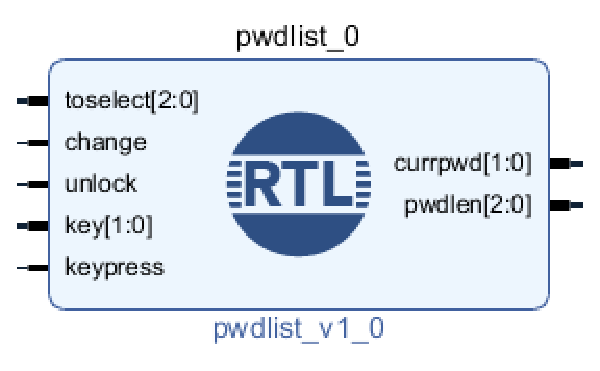
\includegraphics{./images/pwdlist.eps}
    \caption{按键部分}
    \label{fig:by:table}
  \end{minipage}%
  \begin{minipage}[b]{0.5\textwidth}
    \centering
    \begin{tabular}{|c|c|} \hline
      管脚名 & 功能 \\ \hline\hline
      Clk1     &   给密码处理的脉冲信号\\
      Clk2     & 给按键计数器的按键脉冲 \\
      En2      & 修改密码输出使能 \\
      Out1     & 输入密码输出 \\
      Out2     & 修改密码输出 \\
      S0~s3    & 按键输入 \\ \hline
    \end{tabular}
    \caption{功能表}
    \label{table:by:fig}
  \end{minipage}
\end{figure}


\section{总体设计图}


\section{仿真结果}
\subsection{A部分仿真}
\paragraph{仿真激励代码}
\begin{lstlisting}[language={verilog}]
module Test();
reg Press;
reg [1:0]key_in;
wire out;

pwdprocess u0(key_in,3,Press,out);  //预设密码为3

initial begin
Press=0;
key_in=0;
end

always #2 Press=~Press;
always #4 key_in = key_in +1;

endmodule
\end{lstlisting}
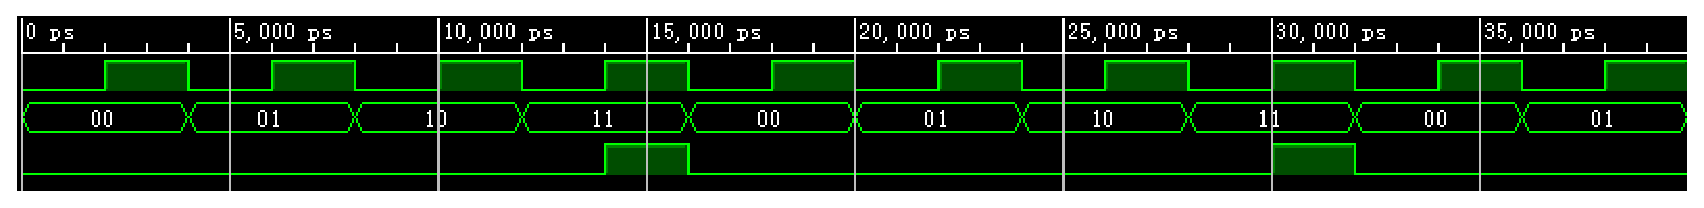
\includegraphics[width=0.9\textwidth]{./images/sim1.eps}

预设的密码为3,经过仿真,输入为3是才能获得正确的脉冲,否则无效。
\paragraph{开锁控制器}
\begin{lstlisting}[language={verilog}]
module Test();
reg [2:0]count;
reg [2:0]length;
wire state;

Lock u0(count,length,state);

initial begin
count=0;
length=5;
end

always #2 count=count+1;

endmodule
\end{lstlisting}
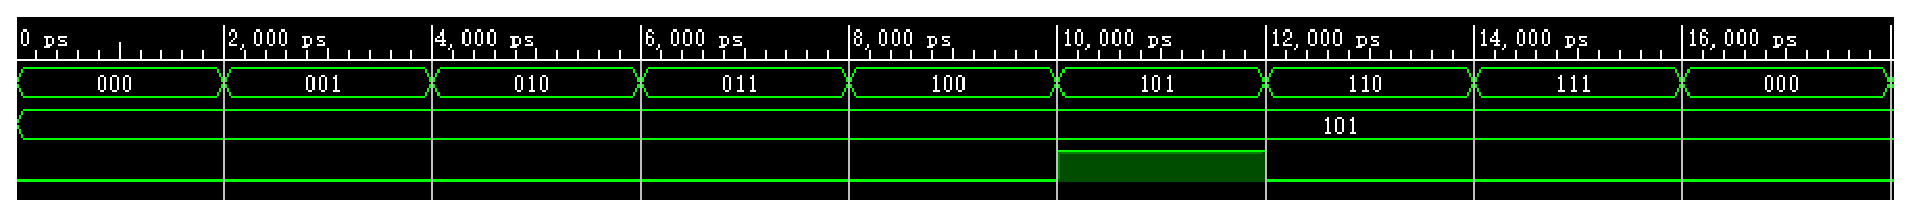
\includegraphics[width=0.9\textwidth]{./images/sim2.eps}

预设的密码长度为5,经过仿真,输入的正确密码为5是才能获得开锁状态。

\paragraph{密码计数器}
\begin{lstlisting}[language={verilog}]
module Test();
reg clk;
reg clr;
wire [2:0]state;

counter u0(clk,clr,state);

initial begin
clk=0;
clr=0;
end

always #2 clk=~clk;

always begin
#35 clr = 1;
#4 clr = 0;end

endmodule
\end{lstlisting}
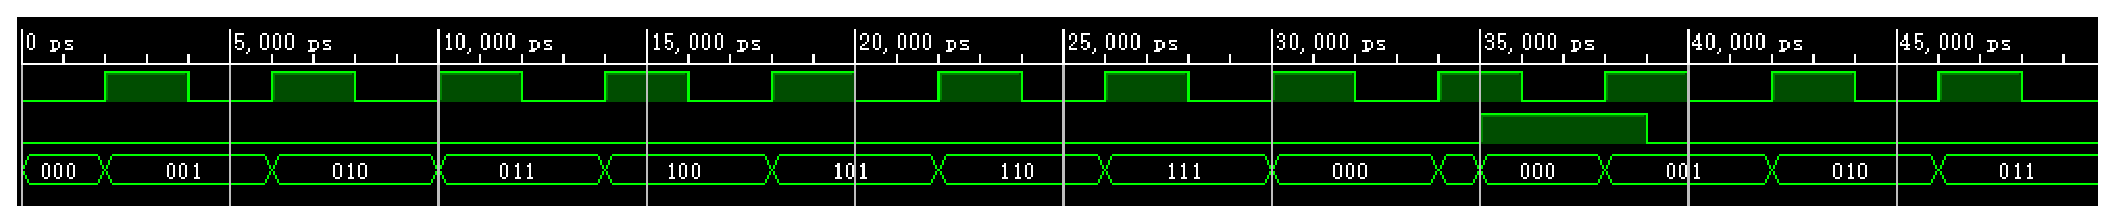
\includegraphics[width=0.9\textwidth]{./images/sim3.eps}

获得一次clk记一次数,上升沿有效,异步清零。

\paragraph{密码表}
\begin{lstlisting}[language={verilog}]
module Test();
reg [2:0]select;        //选择下一位的正确密码
wire [1:0]beSelect;     //被选择出来的密码
wire [2:0]len;          //存储的密码长度

reg change;             //是否修改密码
reg unlock;             //当前开锁状态
reg [1:0]key;           //修改密码所给的值
reg keypress;           //按键脉冲

pwdlist u0(select,beSelect,len,change,unlock,key,keypress);

initial begin
select = 0;
change = 1;
unlock = 1;
key = 0;
keypress = 0;
end

always #2 select=select+1;
always begin
#2 keypress = ~keypress;
key = key + 1;
end

endmodule
\end{lstlisting}
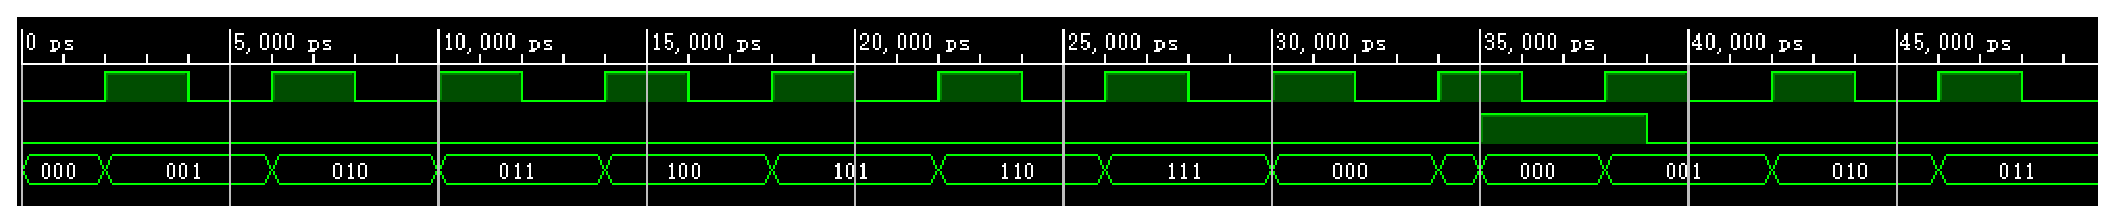
\includegraphics[width=0.9\textwidth]{./images/sim3.eps}

可以修改密码,最多7位,初始密码为0000。

\paragraph{整体仿真}
\begin{lstlisting}[language={verilog}]
module Test();
wire LockState;
reg Change;             //是否修改密码
reg Lock_It;             //当前开锁状态
reg [1:0]KeyValue;           //修改密码所给的值
reg Keypress;           //按键脉冲

Along u0(
    Change,
    Keypress,
    KeyValue,
    Lock_It,
    LockState
    );
initial begin
    Change=0;
    Lock_It=0;
    KeyValue=0;
    Keypress=0;
    //上锁
    #2 Lock_It = 1;
    #2 Lock_It = 0;
    //开锁
    #2 Keypress = ~Keypress;
    #2 Keypress = ~Keypress;
    #2 Keypress = ~Keypress;
    #2 Keypress = ~Keypress;
    #2 Keypress = ~Keypress;
    #2 Keypress = ~Keypress;
    #2 Keypress = ~Keypress;
    #2 Keypress = ~Keypress;
    //修改密码
    #2 Change = 1;
    #2 KeyValue = 3;
    #2 Keypress = ~Keypress;
    #2 Keypress = ~Keypress;
    #2 Keypress = ~Keypress;
    #2 Keypress = ~Keypress;
    #2 Keypress = ~Keypress;
    #2 Keypress = ~Keypress;
    #2 Keypress = ~Keypress;
    #2 Keypress = ~Keypress;
    //密码修改完成,上锁
    #10 Change = 0;
    #2 Lock_It = 1;
    #2 Lock_It = 0;
    //使用新密码开锁
    #2 Keypress = ~Keypress;
    #2 Keypress = ~Keypress;
    #2 Keypress = ~Keypress;
    #2 Keypress = ~Keypress;
    #2 Keypress = ~Keypress;
    #2 Keypress = ~Keypress;
    #2 Keypress = ~Keypress;
    #2 $finish;
end
endmodule
\end{lstlisting}

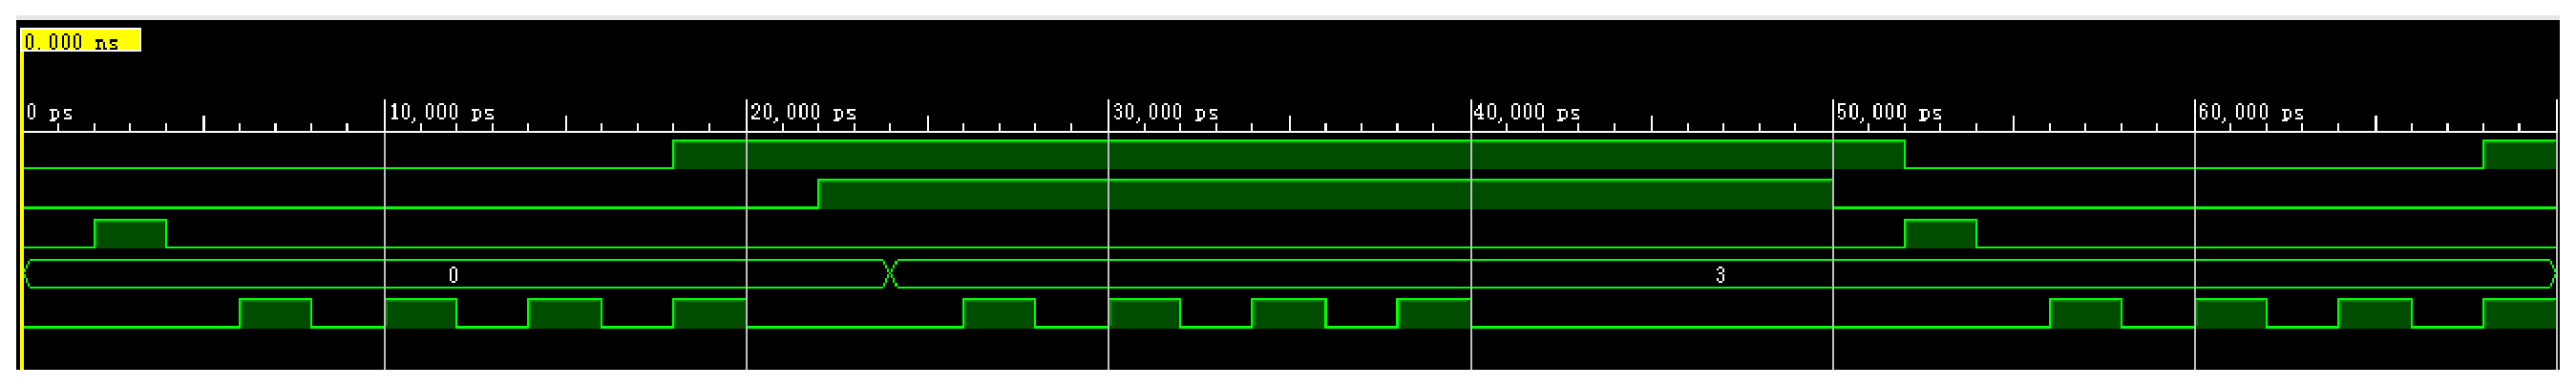
\includegraphics[width=0.9\textwidth]{./images/AlongSimOver.eps}

运行效果良好,开锁上锁,修改密码都做的相当不错。

\subsection{B部分仿真}

\section{工作说明}
\paragraph{冯云龙}密码处理,密码列表,密码计数器,开锁控制器,实验报告。
\subsection{密码处理}
\begin{lstlisting}[language={verilog}]
module pwdprocess(
    input [1:0] keypwd,             //按键输入密码
    input [1:0] cmppwd,             //正确密码
    input keypress,                 //按键脉冲,上升沿触发
    output res                      //输出计数脉冲
    );
    wire cmp;
    assign cmp=keypwd==cmppwd;
    assign res = cmp && keypress;
endmodule
\end{lstlisting}
\subsection{密码表}
\begin{lstlisting}[language={verilog}]
module pwdlist(
    input [2:0]toselect,        //计数选择
    output reg[1:0]currpwd,      //输出密码
    output reg[2:0]pwdlen,       //密码长度
    input change,             //是否修改密码
    input unlock,             //是否已解锁
    input [1:0]key,           //数据输入
    input keypress            //按键脉冲
    );
    reg [15:0]pwd;            //每两位是一组密码.
    reg [2:0]count;

    wire CLK;
    assign CLK = keypress && change && unlock;

    wire Enchange;
    assign Enchange = change && unlock;

    initial begin
    pwd = 0;
    count = 0;
    pwdlen = 4;
    end

    always @(toselect,pwd)
    begin
    case(toselect)
    3'b000 : currpwd = pwd[1:0];
    3'b001 : currpwd = pwd[3:2];
    3'b010 : currpwd = pwd[5:4];
    3'b011 : currpwd = pwd[7:6];
    3'b100 : currpwd = pwd[9:8];
    3'b101 : currpwd = pwd[11:10];
    3'b110 : currpwd = pwd[13:12];
    3'b111 : currpwd = pwd[15:14];
    endcase
    end

    always @(posedge CLK or negedge Enchange)
    begin
    if(Enchange) begin
    case(count)
    3'b000 : pwd[1:0] = key;
    3'b001 : pwd[3:2] = key;
    3'b010 : pwd[5:4] = key;
    3'b011 : pwd[7:6] = key;
    3'b100 : pwd[9:8] = key;
    3'b101 : pwd[11:10] = key;
    3'b110 : pwd[13:12] = key;
    3'b111 : pwd[15:14] = key;
    endcase
    count = count + 1;
    end
    else begin
    if(unlock)
    pwdlen = count;
    count = 0;
    end
    end

endmodule
\end{lstlisting}
\subsection{密码计数器}
\begin{lstlisting}[language={verilog}]
module counter(
    input CLK,                //计数时钟
    input CLR,                //复位
    output reg[2:0]num           //当前计数
    );
    initial num = 0;

    always @(posedge CLK) begin
    if(CLR)
      num = 0;
    else
      num = num + 1;
    end
endmodule
\end{lstlisting}
\subsection{开锁控制器}
\begin{lstlisting}[language={verilog}]
module Lock(
    input [2:0]count,              //当前输入正确的密码个数
    input [2:0]length,             //密码长度
    output state              //当前解锁状态,1为开锁
    );
    assign state = (count == length);
endmodule
\end{lstlisting}
\paragraph{赖昕}计时器,按键计数器,按键译码处理器,显示器。

\end{document} 